\documentclass[oneside,a4paper,12pt]{article}
\usepackage{graphicx}
\usepackage{amsmath}
\usepackage{listings}
\usepackage{array}
\usepackage{subcaption}
\usepackage{caption}
\graphicspath{{~/templates/}, {../images/}}

\makeindex
\begin{document}
	\begin{titlepage}
		\includegraphics[width=4cm]{logopopo.png}
		\hspace*{\fill}
		\includegraphics[width=6cm]{logouniv.png}
		
		\begin{center}
			\vspace{1cm}
			\textbf{Mémoire de Stage de 4e année}\\
			\vspace{1cm}
			\textbf{\LARGE FL-Minifer}\\
			\textbf{\large A Tool To Minify and Unify AdBlocker’s Filter Lists}\\
			\vspace{1cm}
			\textbf{Maxence NEUS}\\
			\vspace{1cm}
			\begin{tabular}{ c c }
				
\includegraphics[width=6cm]{logoInria.jpg} & 
\includegraphics[width=6cm]{logospirals.png}\\
			\end{tabular}

			\vspace{2cm}

			\begin{tabular}{ m{6cm} | m{6cm} }
				\textbf{Polytech Lille} & \textbf{Inria} \\
				\hline
				& \\
				Secrétariat - Bureau & 40 Av. Halley \\
				Boulevard Paul Langevin - Cité Scientifique & 59650 Villeneuve d'Ascq \\
				59655 VILLENEUVE D’ASCQ CEDEX & Tuteur Entreprise : \\
				03-28-76-73-60 & \textbf{Walter RUDAMETKIN} \\
				03-28-76-73-61 & Tuteur Ecole \\
				\includegraphics[width=2.5cm]{logouniv.png} \includegraphics[width=2.5cm]{logopopo.png} & \textbf{Walter RUDAMETKIN} \\
				
			\end{tabular}
			
			\vspace{\fill}
			\textbf{2022}\\
		\end{center}
	\end{titlepage}

\tableofcontents

\newpage

\begin{figure}[h]
	\centering
	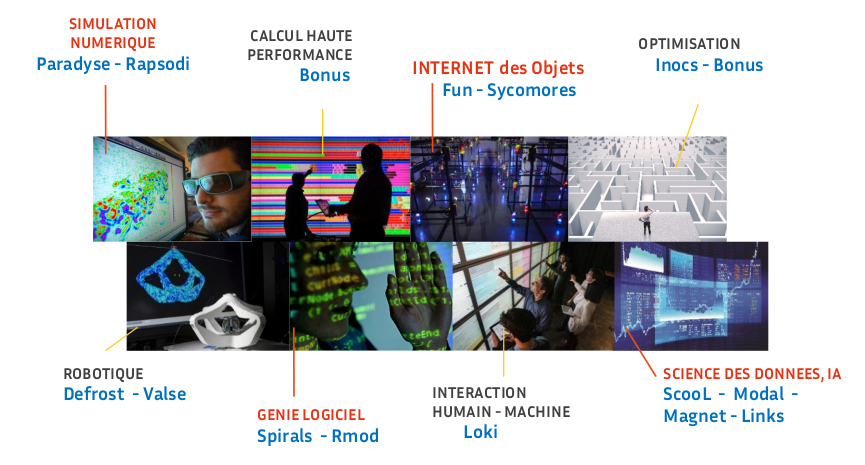
\includegraphics[width=0.55\textwidth]{equipesCentre.png}
	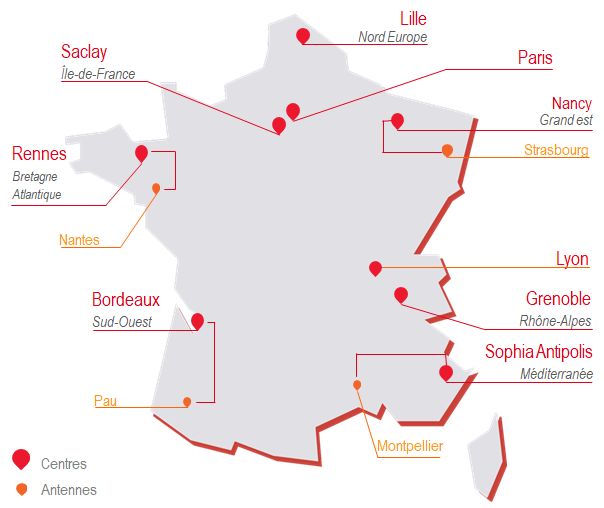
\includegraphics[width=0.4\textwidth]{cartecentres.png}
\end{figure}

\section{Présentation de l'entreprise} \label{PresentationInria}

\subsection{Inria}
Le centre de recherche Inria fondé en 1967 est un établissement publique de recherche se spécialisant dans le domaine des mathématiques et de l'informatique.\\ 
Le centre de Lille Nord Europe fait partie des 9 centres autour de la France et comporte deux complexes: à la Haute Borne et à Euratechnologie. 
Au sein du centre dirigé par Mireille R\'EGNIER operent 15 équipes dont mon équipe d'acceuil: SPIRALS. 

\begin{figure}[h]
	\centering
	
\includegraphics[width=10cm]{direction.png}
	\caption{\'Equipe de direction}
\end{figure}

\subsection{SPIRALS} est une équipe jointe de l'INRIA et de CRISTAL qui se focalise sur les systèmes distribués et l'ingéniérie système. les projets de l'équipe comportent l'étude de solutions autonomes, efficaces et adaptatives pour la récupération et le traitement de données. Dirigée par Lionel Seinturier, l'équipe est actuellement composée de 11 chercheurs permanents, 7 postdocs, 17 doctorants et 7 ingénieurs.


\appendix

\newpage

\begin{center}
	
	\vspace{2cm}
	\renewcommand{\abstractname}{Résumé}
	\begin{abstract}
	
	Lors de ce stage blablabla

	\end{abstract}
	\vspace{\fill}	
	\renewcommand{\abstractname}{Abstract}
	\begin{abstract}
	
	During this internship blablabla

	\end{abstract}

	\vspace{2cm}

\end{center}





\end{document}